%% file: VaBlaetter.tex
%% author: Martin Koelbl
%% date: 1.08.2015
%% purpose: Va-Blaetter Herbst 2015 Hauptdatei

%% Flag, das anzeigt, ob vorlaeufige oder final-Version erstellt wird:
\newif\ifDraft\Draftfalse

%% Flag das anzeigt ob eine Kurzversion erstellt wird:
%% Kurzversion derzeit noch kaum implementiert.
\newif\ifKurzversion\Kurzversionfalse
%\Kurzversiontrue
%% Flag das anzeigt ob Links erstellt werden:
%% Vorsicht: Wenn \Linksfalse eingestellt wird, dann die Datei fktana.ind loeschen und neu erstellen (mit makeindex), sonst beisst sich LaTeX die Zaehne aus.
\newif\ifLinks\Linkstrue
%\Linksfalse


%% Umgebungs-Einstellungen laden, falls vorhanden:
\InputIfFileExists{env_settings.tex}{}{}

%% Dokument-Beschreibung:
%% file: header.tex
%% author: Patrick Leyendecker
%% date: 23.08.2012
%% purpose: Va-Blätter Header nach Vorlage des Skriptenprojekts

\ifDraft
  \global\def\Draftoption{,draft}
\else
  \global\def\Draftoption{}
\fi
%\documentclass[a4paper,12pt,ngerman\Draftoption,twoside]{scrartcl}%,\driver
\documentclass[a4paper,12pt,ngerman,twoside]{scrartcl}

\usepackage[utf8]{inputenc}
%\usepackage[OT2, T1]{fontenc}
\usepackage[ngerman]{babel}

\usepackage{fancyhdr}
\usepackage{amsmath}
\usepackage{xcolor}
\usepackage{graphicx}
\usepackage{paracol}

\usepackage[inner=22mm, outer=26mm, bottom=0mm, top=0mm,footskip=40mm]{geometry}  
\usepackage{textcomp}

 % Seiten-Layout
\usepackage{verbatim}
\usepackage{array}
\usepackage{multicol}
\usepackage{multirow}
\usepackage{eurosym}
\usepackage{blindtext}
\usepackage{lipsum}
\usepackage{soul}
%\usepackage{ulem}
\usepackage{wrapfig}
\usepackage[absolute]{textpos} 
\usepackage{subfigure}
\usepackage{caption}
%\usepackage{subcaption}
\usepackage{dblfloatfix}

%\usepackage{cyrillic}
\usepackage{graphicx}
\newcommand{\heart}{\ensuremath\heartsuit}

\geometry{vmargin={3cm,4cm}}


\makeatother
%% subsubsections nicht mehr nummerieren:
\setcounter{secnumdepth}{1}
%% subsubsections nicht ins Inhaltsverzeichnis:
\setcounter{tocdepth}{1}

\setlength{\parindent}{0pt}

%% Nummerierung von Abbildungen und Tabellen:
\numberwithin{figure}{section}
\numberwithin{table}{section}

\addtokomafont{caption}{\itshape}
\renewcommand*{\figureformat}{}
\renewcommand*{\captionformat}{}

\setlength{\headheight}{26pt}

\setlength{\columnsep}{30pt}

\setlength{\parskip}{6pt}

% Disable single lines at the start of a paragraph (Schusterjungen)
\clubpenalty = 10
%
% Disable single lines at the end of a paragraph (Hurenkinder)
\widowpenalty = 10000
\displaywidowpenalty = 10




\pagestyle{fancy}
% \fancyfoot{}
\fancyhead{}
\fancyhead[EL,OR]{ \footnotesize Seite \thepage \\ Die Vandalenblätter}
\fancyhead[ER,OL]{\footnotesize 130/2025 } %\\ (Nummer 32 -- Herbst
% 2014)}
\fancyhead[EC,OC]{ \large \textsc{\leftmark } \vspace{0pt}}

\renewcommand{\thesection}{}
\renewcommand{\theparagraph}{}
\renewcommand{\thesubsubsection}{}
\renewcommand{\sectionmark}[1]{\markboth{#1}{}}

\makeatletter
\newenvironment{tablehere}
  {\def\@captype{table}}
  {}

\newenvironment{figurehere}
  {\def\@captype{figure}}
  {}
\makeatother


%% Makros und Umgebungen:
%%% file: makros.tex
%% author: Thomas Satzger
%% date: 08.03.2007
%% purpose: Diplomarbeit, LaTeX-Definitionen


%% Theorem-Umgebungen:

%% Nummerierung nach sections, alle Theoreme mit dem gleichen Zaehler:
\theorembodyfont{\rmfamily}
\theoremstyle{break}% neue Zeile nach Theoremueberschrift
\newtheorem{defi}{Definition}[section]
\newtheorem{lemma}[defi]{Lemma}
\newtheorem{satz}[defi]{Satz}
\newtheorem{kor}[defi]{Korollar}
\newtheorem{bem}[defi]{Bemerkung}
\newtheorem{bemerkung}[defi]{Bemerkung}
\newtheorem{bemerkungen}[defi]{Bemerkungen}
\newtheorem{beispiel}[defi]{Beispiel}
\newtheorem{beispiele}[defi]{Beispiele}
\newtheorem{nothing}[defi]{\hspace{-1ex}}% Umgebung ohne Ueberschrift
%% TODO: nothing schaut furchtbar aus.


%% Umgebungen ohne Nummer:
% \input thbnone.sty
% \theoremstyle{bnone}% wie break, nur ohne Nummer
%\newtheorem{defi*}{Definition ohne Nummer}[section]
\newtheorem{beispiel*}{Beispiel}[section]
\newtheorem{beispiele*}{Beispiele}[section]
\newtheorem{bem*}[beispiel*]{Bemerkung}
\newtheorem{bemerkung*}[beispiel*]{Bemerkung}
\newtheorem{bemerkungen*}[beispiel*]{Bemerkungen}
\newtheorem{folgerung}[beispiel*]{Folgerung}
\newtheorem{folgerungen}[beispiel*]{Folgerungen}
%% Beweis:
%% qed-Kaestchen wird automatisch gesetzt, ausser es wurde schon 
%% von Hand (per \qed) gesetzt.
%% Ist eine Liste am Ende vom Beweis (d.h. itemize/enumerate/description),
%% dann muss \qed nach dem letzten Text (von Hand) eingefuegt werden.
\newtheorem{beweis}[beispiel*]{Beweis}
\let\tmpendbeweis=\endbeweis
\def\endbeweis{\smartqed\tmpendbeweis}


%% QED-Kasterl. Am sinnvollsten am Ende eine Absatzes
%% Klappt im Mathemodus nicht so toll.
\newif\ifQed\Qedfalse % speichern, ob manuell qed gesagt wurde 
%% (damit bei \end{beweis} nicht noch ein qed dazu kommt)
\newcommand{\qed}{\nolinebreak[4]\hfill\rule{1.2ex}{1.2ex}\global\Qedtrue}% 
%% qed, dass nur bei \Qedfalse gesetzt wird (fuer Beweisumgebung):
\newcommand{\smartqed}{\ifQed\relax\else\qed\fi\global\Qedfalse}


%% Keine Beweise, Beispiele in der Kurzversion:
%% TODO: Hier kann man noch optimieren (Beispiele rauslassen geht noch nicht).
\ifKurzversion
  \let\beweis=\comment
  \let\endbeweis=\endcomment
\fi


%% enumerate- und itemize-Umgebungen anpassen:
\partopsep=-\parskip% wirkt bei Absaetzen vor enumerate
\let\tmpenumerate\enumerate
\def\enumerate{\par%\vspace{-\topsep}
\vspace{-\parskip}%
\vspace{-\partopsep}%
\tmpenumerate\partopsep=0mm\itemsep=0mm\parsep=0mm}

%% Zwei neue Umgebungen f�r Listen: lista mit Buchstabenz�hlung, und listi mit r�mischen Zahlen
%% muss noch entwickelt werden
\newcommand{\listea}{\begin{enumerate}[\medspace (a)]}
\newcommand{\listeaend}{\end{enumerate}}
\newcommand{\listei}{\begin{enumerate}[\medspace $(i)$]}
\newcommand{\listeiend}{\end{enumerate}}
\newcommand{\liste}{\begin{enumerate}[\medspace 1.]}
\newcommand{\listeend}{\end{enumerate}}

\newcommand{\nobr}{\nolinebreak}

\newcommand{\vo}{ v\//\/o }


%Operatoren
%\DeclareMathOperator{\rang}{rang}
%\DeclareMathOperator{\sgn}{sgn}

% \vecn - Allgemeiner 1xn-Spaltenvektor mit Klammern ausnrum
% F�r Zeilenvektoren nimmt man besser \mat (siehe unten)
% Beispiel: \vecn{a \\ b \\ c}
%\newcommand{\vecn}[1]
%{\left(\begin{array}{c} #1 \end{array}\right)}

% \closure{TEXT} macht einen �berstrich �ber den TEXT,
% Denke an den Abschluss von Mengen
\newcommand{\closure}[1]
{\overline{#1}}

% \mat{SPALTEN}{INHALT} - Matrizen (mit normalen  ( ) )
% Beispiel: \mat{cc}{a & b \\ c & d}
\newcommand{\mat}[2]
{\left(\begin{array}{#1} #2 \end{array}\right)}

% \detmat{SPALTEN}{INHALT} - Determinanten-Matrizen ( | | statt ( ) )
% Syntax wie bei \mat
%\newcommand{\detmat}[2] % det ist leider vergeben
%{\left|\begin{array}{#1} #2 \end{array}\right|}

% \gmat{SPALTEN}{INHALT} - Matrizen mit geschweiften Klammern ( { } statt ( ) )
% Syntax wie bei \mat
\newcommand{\gmat}[2] % det ist leider vergeben
{\left\{\begin{array}{#1} #2 \end{array}\right\}}


%% Skalarprodukt:
%% Das Argument steht zwischen den Klammern.
\def\skalar#1{\ensuremath{\left\langle #1\right\rangle}}

%% Absolutbetrag (einfache senkrechte Striche, 
%% Groesse automatisch angepasst):
%% TODO: In chapter2.tex ab section 5 einfuegen.
\newcommand{\abs}[1]{\ensuremath{\left|#1\right|}}

%% Norm (doppelte senkrechte Striche, Groesse automatisch angepasst):
\def\norm#1{\ensuremath{\left\|#1\right\|}}

%% Erzeugendensystem einfach und doppelt
\def\erz#1{\ensuremath{\left\langle #1\right\rangle}}
\def\erzerz#1{\ensuremath{\left\langle\left\langle #1\right\rangle\right\rangle}}

%% Stacked Equal: = mit einem mathrm-Text dr�ber
\newcommand{\smequals}[1]
{\stackrel{\mbox{\tiny #1}}{=}}

\newcommand{\smany}[2]
{\stackrel{\mbox{\tiny #1}}{#2}}


% Personen-Namen werden in guten B�cher in Kapit�lchen geschrieben
\newcommand{\name}[1]{\textsc{#1}}


%% Mathe-Pfeile:
% Langer �quivalenzpfeil mit Abst�nden:
\def\aequiv{\ensuremath{\ \Longleftrightarrow\ }\xspace}
% Langer Implikationspfeil mit Abst�nden:
\def\impl{\ensuremath{\ \Longrightarrow\ }\xspace}
% Definitions�quivalenzpfeil mit Abst�nden:
\def\define{\ensuremath{\ :\Longleftrightarrow\ }\xspace}
% Beweis, Hin-Richtung und R�ck-Richtung:
% Verwendung: 
%\begin{description}\item[\hin]...\item[\rueck]...\end{description}
\def\hin{\glqq$\Longrightarrow$\grqq{}}
\def\rueck{\glqq$\Longleftarrow$\grqq{}}
% Geschweifte Klammer mit Kommentar unter Formeln:
% Zuerst den tiefgestellten Text, dann den normalen.
\def\underbraced#1#2{\ensuremath{\underset{\rule{0mm}{1.5ex}\makebox[0mm]{$\scriptstyle #1$}}{\underbrace{#2}}}}
% Transponiert:
%\def\trans{^{\mathsf T}}
\def\trans{^{\mathrm T}}

% Orthogonal
\def\ortho{^{\bot}}


%% TODO-Makro:
\def\todo#1{\ifDraft\par{\bfseries TODO: #1}\par\fi}
%% Marke zum Bild einfuegen, Argument ist z.B. Bildbeschreibung (caption):
\def\bild#1{\todo{Bild: #1}}


%% Makros spezifisch fuer Funktionalanalysis:
% Topologie (Schreibschrift-T):
\def\topo{\ensuremath{\mathcal T}}
% Bidual: Setzt zwei hochgestellte Sterne.
\def\bidual{\ensuremath{^{\ast\ast}}}

% URL einf�gen
\DeclareRobustCommand{\urlformat}[1]{\url{#1}} 

%% Bilder einfuegen:
%% Syntax:
%%   \abbildung{dateiname}[graphicx-optionen]{Beschriftung}[label]
%% Argumente: Dateiname (ohne Pfad und Endung), 
%% Optionen fuer includegraphics (optional), 
%% caption, Label (optional).
%% Beispiele:
%% \abbildung{hausdorff}{Zur Hausdorff-Eigenschaft}
%% \abbildung{hausdorff}{Zur Hausdorff-Eigenschaft}[fig:hausdorff]
%% \abbildung{hausdorff}[height=5cm,width=\textwidth,keepaspectratio=]{Zur Hausdorff-Eigenschaft}
\def\bilderpfad{./bilder/}
%\ifthenelse{\equal{\driver}{pdftex}}%
%  {\global\def\bildendung{.pdf}}%
%  {\global\def\bildendung{.ps}}% 
\makeatletter
\def\abbildung#1{\@ifnextchar[{\@bbildung{#1}}{\@bbildung{#1}[scale=1]}}
\def\@bbildung#1[#2]#3{%
  \@ifnextchar[{\@bbild@ngl{#1}[#2]{#3}}{\@bbild@ng{#1}[#2]{#3}}}
\def\@bbild@ng#1[#2]#3{%
  \begin{figure}[htb]
    \begin{center}
      \includegraphics[#2]{\bilderpfad#1}%\bildendung
      \caption{#3}
    \end{center}
  \end{figure}}
\def\@bbild@ngl#1[#2]#3[#4]{%
  \begin{figure}[htb]
    \begin{center}
      \includegraphics[#2]{\bilderpfad#1}%\bildendung
      \caption{#3}
      \label{#4}
    \end{center}
  \end{figure}}
\makeatother




\def\Input{\item[\textbf{Input: }]}
\def\Output{\item[\textbf{Output: }]}
\def\comment{\%}
\def\Given{\item[\textbf{Gegeben: }]}
\def\False{\ensuremath{\text{\bfseries False}}}
\def\True{\ensuremath{\text{\bfseries True}}}
\def\return{\ensuremath{\text{\bfseries Return}}}

\def\var#1{\ensuremath{\textit{#1}}}
%\renewcommand\algorithmiccomment[1]{ \{#1\}}%


\renewcommand\appendix{\par
\setcounter{section}{0}%
\setcounter{subsection}{0}%
\setcounter{figure}{0}
\renewcommand\thesection{\Alph{section}} %
\renewcommand\thefigure{\Alph{section}.\ arabic{figure}}} 



%% Zwei neue Umgebungen für Listen: lista mit Buchstabenzählung, und listi mit römischen Zahlen
%% muss noch entwickelt werden
% \newcommand{\listea}{\begin{enumerate}[\medspace (a)]}
% \newcommand{\listeaend}{\end{enumerate}}
% \newcommand{\listei}{\begin{enumerate}[\medspace $(i)$]}
% \newcommand{\listeiend}{\end{enumerate}}
% \newcommand{\liste}{\begin{enumerate}[\mAnonymer Barbetriebedspace 1.]}
% \newcommand{\listeend}{\end{enumerate}}

\newcommand{\nobr}{\nolinebreak}
\newcommand{\vo}{v\//\/o }
%\newcommand{\tocline}[1]{\addtocontents{toc}{\contentsline {section}{\numberline{}{\hspace{-0.5cm}{\large {#1}}}}}}
\newcommand{\tocline}[1]{\addtocontents{toc}{section}{\numberline{}\hspace{-0.5cm}{\large {#1}}}}
% select ONE of the two following lines to switch between color and bw pictures
\newcommand{\Bilder}{Bilder}
%\newcommand{\Bilder}{Bilder/farbig}

\newcolumntype{P}[1]{>{\centering\arraybackslash}p{#1}}


%\makeindex
\pagenumbering{arabic}


\begin{document}

%% Titelseite:

\begin{titlepage}

%\Huge Dummy für Titelseite

\begin{textblock}{3}(0,0) 
     \includegraphics[width=1.\paperwidth]{Titelseite/130Titlepage}
\end{textblock} 

\end{titlepage}

\leavevmode\newpage


%% Disclaimer:
%\input disclaimer.tex

\clearpage


%% Inhaltsverzeichnis:
%\linespread{1}

% Zeilenabstand im Inhaltsverzeichnis:
\addtocontents{toc}{\protect\linespread{+0.2}\protect\selectfont}

\tableofcontents
\enlargethispage{1cm}

\clearpage


%%%%%%%%%%%%%%%%%%%%%%%%%%%%%%%%%%%%%%%%%%%%%%%%%
%% Teil WS1819

%\section*{Wintersemester 2024/2025}
\sectionmark{Impressum}

\enlargethispage{1cm}

%\vspace*{5mm}
\begin{figurehere}
 \begin{center}
   %\includegraphics[width=0.8\hsize]{Bilder/chargen/chargen3.JPG}
   \includegraphics[width=0.8\hsize]{Bilder/chargen/chargen3.jpg}
   
   \caption{Das Chargenkabinett des WS 24/25}
 \end{center}
\end{figurehere}

%\vspace*{.5cm}

%\textbf{Chargenkabinett des WS 2024/2025} \vspace*{1cm} \\
\vbox{
	\begin{tabular}[h]{*5{c}}
		Scriptor & Fuxmajor & Senior & Consenior & Kassier\\
		\textbf{Benedikt Kirchhof} & \textbf{Magnus Weig} & \textbf{Raphael Frank} & \textbf{Elia Strasser} & \textbf{Felix Hantke} \\
		\textit{stud. paed.} & \textit{stud. el.} & \textit{stud. inf.} & \textit{stud. rer. oec.} & \textit{stud.paed.}\\
	\end{tabular}
}

\vspace{2mm}
%\subsection*{Semestermotto des WS 2024/2025}
\begin{LARGE}
	\begin{center}
		\glqq Wer nichts weiß, muss alles glauben\grqq
	\end{center}
%	\hspace*{2cm}\glqq Tradition soll ein Sprungbrett sein,\\
%    \hspace*{7cm} aber kein Ruhekissen.\grqq
\end{LARGE}

\vspace*{-3mm}
- \textit{Marie von Ebner-Eschenbach}

\vspace*{7mm}
\begin{minipage}[h!]{160mm}
	\small{
		\textbf{Impressum}
		
		Vandalenblätter 130/2025, Ausgabe WS 2024/25
		
		Mitteilungsblatt der K.D.St.V. Vandalia Prag zu München im CV
		
		Namentlich gekennzeichnete Beiträge stellen keine redaktionelle Meinungsäußerung dar. Die Redaktion behält sich vor, Änderungen vorzunehmen, die den Sinn des Textes wahren.
		\\
		\newline
		\vspace{6pt}
		\noindent\begin{tabular}{ll}
			Titelbild: & Philipp Keyzman\\
			Lizenz: & Creative Commons 2.0 \\
			Satz \& Layout: & Philipp Keyzman, Alessandro Samuelli und Leonard Rothe mittels
			\LaTeX
			\\
			Bildmaterial: & Elias Haindl\\
			Druck: & https://www.wir-machen-druck.de\\
			Auflage: & 500 Stück\\
			Redaktionsanschrift: & Vandalenblätter-Redaktion \\	
			& c/o K.D.St.V. Vandalia\\
			& Friedrichstraße 34, 80801 München\\
			& vablaetter@vandalia.de
		\end{tabular}
	}
	
\end{minipage}
\clearpage

\clearpage


%%%%%%%%%%%%%%%%%%%%%%%%%%%%%%%%%%%%%%%%%
%% Vorworte

\section{Vorwort des Philisterseniors}
\sectionmark{Vorwort des Philisterseniors}

%\begin{figurehere}
%	\begin{center}
%		\includegraphics[width=\linewidth]{Bilder/andechs2.jpg}
%%		\caption{xxx} 
%	\end{center}
%\end{figurehere}

\begin{multicols}{2}

Die Jahreshauptversammlung des CV fand in diesem Jahr in Berlin statt. Sie war geprägt durch eine Diskussion über unser Prinzip religio. Der ein oder andere hat davon vielleicht in der ACADEMIA etwas gelesen. Die Diskussionen waren auch in den vorausgegangenen Regionaltagungen zum Teil sehr hitzig. Ohne die Details hier auszubreiten, möchte ich aber einen kurzen Blick darauf werfen. Die Tatsache, dass ein Vorort seine Amtszeit dadurch prägen will, etwas zu verändern und dann nicht bis zur CV damit wartet, sondern bereits zu Beginn seiner Amtszeit einen Diskurs startet, halte ich für richtig. Jedes Chargenkabinett - sei es im Vorort oder auch in der Verbindung - hat eine zeitlich begrenzte Amtszeit. Veränderungsprozesse am Ende der Amtszeit zu starten, sind zumeist sinnlos. Aus dieser Sicht betrachtet, war das Vorgehen des Vororts Berlin sehr gut geplant und kann und sollte ein Vorbild für zukünftige Chargenkabinette sein.
Über den Inhalt wird und wurde trefflich diskutiert und gestritten. Aus meiner Sicht gibt es hier durchaus gute Impulse. Über andere Thesen darf und muss man auch geteilter Meinung sein. Wichtig scheint mir aber, dass wir Themen und auch unsere Prinzipien diskutieren. Ohne Diskussion über unsere Prinzipien und wie wir sie auch in Zukunft leben, stellt sich jedem von uns über kurz oder lang die Frage nach der Bedeutsamkeit unseres Verbandes.
Gute Diskussionen über strittige Themen können verbinden, das Profil stärken und sollten uns als akademischen und katholischen Verband ausmachen. Als wichtige und beruhigende Botschaft aus diesen Diskussionen ist mir unser einigendes Motto immer wieder lebendig vor Augen geführt worden: \glqq In necessariis unitas, in dubiis libertas, in omnibus caritas\grqq!
Der zentrale Punkt ist mir aber, dass hinter diesen Diskussionen spürbar ist, dass es Cartellbrüder gibt, denen unser Verband und unsere Verbindungen wichtig sind. Heute ist das für mich ein stärkender Impuls entgegen der weitverbreiteten Egozentrik und Selbstoptimierung in unserer Gesellschaft.
Ich würde mich freuen, wenn wir auch im Jahr unseres 120. Gründungs- und Stiftungsfests aktiv über die Weiterentwicklung unserer Vandalia sprechen und diskutieren. Was bedeuten unsere Prinzipien für uns auch im 21. Jahrhundert! Diese Auseinandersetzung in bundesbrüderlicher Freundschaft ist für ein “vivat, crescat, floreat at multos annos Vandalia” unbedingt notwendig! 

\end{multicols}
\begin{flushright}
		\hfill\emph{Dr. Michael Spickenreuther Va!}
	\end{flushright}
\newpage

\section{Vorwort des Seniors aus dem WS 2023/24}
\sectionmark{Vorwort des Seniors}

Liebe Freunde der Vandalia,\\
Liebe Bundesbrüder,
\begin{multicols}{2}

Es ist mir eine Freude, Dir die neuste Ausgabe der Vandalenblätter vorstellen zu dürfen. Dank gilt dabei vor allem den Redakteuren dieser Ausgabe, den Bundesbrüdern Philipp Keyzman und Benedikt Kirchhof, welche diese Ausgabe zusammengestellt haben und gegen viele Widrigkeiten die Prozesse, die hierfür notwendig sind, wiederbelebt oder gar neu erfunden haben. So hoffe ich, dass die Artikel Dir einen guten Einblick in das vergangene Wintersemester geben können und auch bei den Bundesbrüdern, welche daran aktiv teilgenommen haben, so manche schöne Erinnerung wieder hervorruft. An dieser Stelle möchte ich - auch stellvertretend für die Redaktur - Dich nochmal herzlich dazu einladen, gerne auch Deine eigenen Beiträge einzusenden. Ob Du aus Deiner akademischen Arbeit, Deinem Alltag, einer spannenden Reise berichten oder einfach einen Kommentar zum aktuellen Geschehen in der Verbindung und Welt verfassen möchtest: Gerne nehmen wir diese Artikel oder auch photographischen Interpretationen in die Blätter auf und fördern so den Austausch zwischen den Bundesbrüdern. Hierfür sind die Redakteure in Zukunft unter \textbf{vablaetter@vandalia.de} erreichbar, sodass die Artikel auch eine Amtsübergabe überdauern werden.

Zuletzt möchte ich Dir noch kurz die Chargen des vergangenen Wintersemesters 2023/24 vorstellen und anschließend einen kurzen Überblick über dieses geben. Als Kassier und Schriftführer konnten die Bundesbrüder Daniel Rampf und Raphael Frank erste Erfahrungen in der Chargenarbeit gewinnen. Sie wurden zusammen mit ihrem Leibbruder Elia Strasser auf dem Gründungsfestkommer geburscht. Die gesammelte Erfahrung prädestiniert sie dafür, in Zukunft auch höhere Verantwortung für unsere liebe Vandalia zu übernehmen. Als Fuxmajor kümmerte sich Bundesbruder Fabian Heinrich in seiner vierten Charge um die Keilarbeit sowie die Erziehung des Fuxenstalls. Der Hohe Consenior, Bundesbruder Derek Dominguez, kam im WS 2022/23 als ZM zu unserer Vandalia. Zuvor besuchte er in Hamburg das Studienkolleg und wurde im WS 2021/22 bei e.V. K.D.St.V. Wiking Hamburg rezipiert. Er bereicherte das Semester und insbesondere die Begrüßungsabende durch Gerichte aus seiner ecuadorianischen Heimat. Als Senior durfte ich, Konrad Schönleber, wie bereits im Sommersemester unserer lieben Vandalia vorstehen.
\\
Das Semester stand unter dem Wahlspruch \textit{"Wo sich Männr finden, die für Ehr und Recht, mutig sich verbinden, weilt ein frei Geschlecht"}. Dieses Zitat aus dem Gedicht "Freiheit, die ich meine" von dem Dichter Max von Schenkendorf wurde etwa in einigen Kneipreden erörtert. Neben diesen obligatorischen Kneipen fand im Semester auch eine Rezeptionskneipe statt. Es wurden auf jenen Veranstaltungen sieben Füxe rezipiert, von welchen uns leider im Laufe des Semesters zwei verlassen mussten, sodass sich der Fuxenstall mit nun fünf Füxen doch adäquat gefüllt zeigt. Höhepunkt des Semesters war das vom 24. bis 26. November stattfindende 119. Gründungsfest. Dieses war herausragend besucht und wir hatten die Ehre, den 1. Vizepräsidenten aD des Bayrischen Landtags, Karl Freller hierzu als Festredner begrüßen zu dürfen. Das Grundprinzip der religio war unter anderem durch Besuche der Roratemessen oder auch dem Pater-Rupert-Mayer-Gedächtnisgottesdienst vertreten. Auch die scientia kam mit verschiedenen Vorträgen und Museumsbesuchen nicht zu kurz. Neben der Feuerzangenbowle fand auch eine familiäre Adventsfeier als eine winterliches Äquivalent des Maifests statt. Hierzu wurde zwar eine größere Menge an Gebäck gebacken, allerdings konnte sie wegen Krankheit vieler Bundesbrüder nur in recht kleinem Kreise stattfinden. Man könnte sie vermutlich in den kommenden Jahren mit wenig Aufwand zu einer größeren Veranstaltung ausbauen, wenn man dies den Bundesbrüdern besser kommunizieren würde. Anfang November gab es zudem schon ein frühes, kleines Feierwochenende: Bei einem zweitägigen Tanzkurs wurden die Kenntnisse der Bundesbrüder für die kommende Ballsaison aufgefrischt. Zudem durften wir uns an diesem Samstag den den Genuss einer Martinsgans kommen. Hierfür gilt mein Herzlicher Dank an Fbr. Rampf e.V. K.St.V. Rechberg sowie an seine Frau für die sehr lehrreiche Durchführung des Tanzkurses und an unsere Bundesbrüder AH Michael Oppitz sowie AH Richard Gurtner, welche das Martinsgansessen organisiert und mit bester Kochkunst vorbereitet haben.
Doch zu den einzelnen Veranstaltungen kannst Du in den folgenden Artikeln detailliertere und hoffentlich weniger langweilige Worte finden. So bleibt mir nur, meinen Dank an alle Bundesbrüder und insbesondere an die Philisterchargen für die Unterstützung vor und während des Semesters auszusprechen. Ich bin höchst erfreut, dass ich unserer Vandalia zwei Semester vorstehen durfte und hier in der schönsten Stadt am Isarstrande eine zweite Heimat in unserer Verbindung gewinnen konnte.  

Auf dass diese Freude noch vielen weiteren Bundesbrüdern zuteil werden wird:

Vivat, crescat, floreat Vandalia ad multos annos!
	%
	\begin{flushright}
		\hfill\emph{Konrad Schönleber RBo! Va!}
	\end{flushright}
	%
\end{multicols}


\clearpage


%%%%%%%%%%%%%%%%%%%%%%%%%%%%%%%%%%%%%%%%%
%% Berichte aus dem Semester

%\clearpage

%\clearpage

%\clearpage

%\clearpage

%%%%%%%%%%%%%%%%%%%%%%%%%%%%%%%%%%%%%%%%%
%% Magazinteil

\section{Rede des Seniors zur Antrittskneipe}
\sectionmark{Antrittskneipe}
Werte Kneipcorona,
\begin{multicols}{2}

Ein neues
Semester beginnt. Der aufmerksame Bundesbruder dürfte es bereits daran erkannt
haben, dass er sich auf einer Semesterantrittskneipe befindet. Andere haben
bereits die ersten Vorlesungen besucht. Und doch erkennt man es auch an etwas
anderem. Es ist nichts Konkretes wie ein Kalendereintrag oder ein Wecker, der
um 6 Uhr klingelt, nachdem ein heiterer Abend erst um 2 Uhr sein Ende fand. Und
doch kann man es anhand vieler Eindrücke spüren.

Zuallererst
finden nach dem meiner Meinung nach sehr gut gelungenen Ferialprogramm nun auch
wieder Semesterveranstaltungen statt – sei es der Antrittsgottesdienst der
Katholischen Hochschulgemeinde, der wirklich sehr gut besucht wurde, oder unser
kommender Begrüßungsabend nächste Woche. Dies sorgt natürlich dafür, dass man
wieder regelmäßig Bundesbrüder auf dem Haus sieht, nette Gespräche führen kann
und das ein oder andere leckere Bier nach einem längeren Uni-Tag gemeinsam
verzehrt.

In meiner
Rede bei unserer Abkneipe letztes Semester erzählte ich von diesem
unzufriedenen Gefühl, das man nach der Klausurenphase hat, obwohl man schon
alle Prüfungen geschrieben hat – und dass dieses Gefühl auch erst einmal
bleibt.

Jedoch bringt ein neues Semester auch immer ein ganz besonderes Gefühl mit sich. Jedes
Semester aufs Neue startet man mit einem unbeschriebenen Blatt, einem Neuanfang
und für die meisten mit neuer Motivation und Energie. Denn auch wenn ein
Semester gefühlt immer sehr schnell vorbeigeht, unterschätzen die meisten, was
sie in einem Semester alles erreichen und schaffen können. Man arbeitet fürs
Studium – da bin ich mir bei den meisten sogar fast sicher –, aber man arbeitet
auch an sich selbst. Man entwickelt sich weiter, knüpft neue Kontakte und ist
selbst nach nur einem Semester doch ein Stück weit ein anderer Mensch. Ich bin
mir sicher, dass auch unsere neuen Füxe diese Motivation und Energie in sich
tragen und wünsche ihnen einen guten Start ins Studium und in unser
Gemeinschaftsleben.

Dieses Semester ist bunt gefüllt mit mehreren Themenabenden wie dem Italienischen
Abend, der Bierauswahl oder dem Martinsgansessen. Wir fahren nach Tübingen auf
Aktivenfahrt und feiern unser\textbf{120. Gründungsfest am 23.11.}, zu dem
ich euch alle sehr herzlich einlade. Auf einige interessante Vorträge folgen
der Musikalische Abend und die große Vandalen-Weihnachtsfeier. Es gibt also
vieles, auf das man sich freuen kann.

In diesem
Sinne freue ich mich auf alles, was unsere Verbindung auch in diesem Semester
blühen, wachsen und gedeihen lässt. Darauf einVivat, crescat,
floreat Vandalia ad multos annos!

Prost, Corona!

	%
	\begin{flushright}
		\hfill\emph{Raphael Frank Va! x}
	\end{flushright}
	%
\end{multicols}


\newpage

\section{Perspektivforum Vandalia - Klausurtagung}
\sectionmark{Perspektivforum Vandalia - Klausurtagung}


\begin{multicols}{2}	

Was heißt Zukunft? Dieser Frage gingen
unsere Vandalen am 26. Oktober 2024 auf dem Perspektivforum nach. Ein
Perspektivforum – das gab es noch nie; das erste seiner Art. Worum ging es? Die
großen Themen der Zukunft: wie sich Vandalia weiterentwickeln will, welche
Rolle wir im Couleurwesen einnehmen, was mit der Deutschen Burse geschieht und
vieles mehr wurden in kleinem, freundschaftlichem Rahmen diskutiert. Mit dabei
waren vor allem Aktive, einige Inaktive und aus der Altherrenschaft Phil-xxx
Guido Herr sowie Bernhard Müller.

Bei einem Perspektivforum kommen keine
Beschlüsse heraus, sondern Vorschläge für Beschlüsse. Keine neuen Regeln,
sondern Reflexionen über Regeln. Es geschieht nichts Verbindliches, sondern
etwas Verbindendes: Man diskutiert gemeinsam, orientiert sich untereinander,
tauscht Ideen aus und nimmt sich die Zeit, die man auf einem Convent
normalerweise nicht hat. Man schaut aus der Vogelperspektive auf die Verbindung
– es geht um die nächsten Jahre und Jahrzehnte, nicht um das nächste Wochenende
oder das kommende Semester.

Ein Perspektivforum liefert, wie der Name
schon sagt, Perspektive: ein genaues Hinsehen auf den aktuellen Zustand und
einen Ausblick darauf, wo es hingehen soll. Eine Rückschau auf die Entwicklung
der Verbindung in den letzten Jahren und eine Vorschau auf die anstehenden
Herausforderungen.

Das Ganze findet zwanglos und in
entspanntem Rahmen statt. Zwischenzeitlich entwickelte sich in den hinteren
Reihen des Kneipsaals sogar eine Tee-Zeremonie. Dennoch haben das Diskutieren
Zeit und Energie gekostet. Sechs Stunden dauerte das Perspektivforum – am Ende
hat die Zeit fast nicht gereicht.

Was dabei herausgekommen ist, darf jeder
gerne beim nächsten Perspektivforum erfahren, wenn das Protokoll der letzten
Sitzung verlesen wird. Nur so viel sei verraten: Vor allem die Attraktivität
der Deutschen Burse, die Zimmervergabe im Wohnheim, die Ansehnlichkeit der
Vandalenräume, der Zustrom neuer Mitglieder, die Beziehung zwischen Aktivitas
und Altherrenschaft sowie das Selbst- und Außenbild der Vandalia waren Themen.
Man sieht: reichlich Stoff zum Nachdenken – und sicherlich Themen, bei denen
der Input von „alten Hasen“ nicht schadet.

Dieser Artikel darf deshalb auch gerne als
Einladung gelesen werden: Wenn das Altherrendasein aus langer Erfahrung und
einem „Vogelblick“ auf das Studentenverbindungswesen besteht, dann ist Input
aus der Altherrenschaft sicherlich begehrt. Vielleicht freut sich das nächste
Perspektivforum also über Zustrom von Jung und Alt. Der nächste Termin ist
voraussichtlich im Wintersemester 2025/26.

	%
	\begin{flushright}
		\hfill\emph{Christian Schnurr Va!}
	\end{flushright}
	%	
\end{multicols}
%

\newpage

\section{Italienischer Abend}
\sectionmark{Italienischer Abend}

\begin{figurehere}
		\begin{center}
			\includegraphics[width=0.8\linewidth]{./Bilder/Neue Bilder/Italienischer Abend//DSC_3481-min}
		\end{center}
	\end{figurehere}

\begin{multicols}{2}

Dieses Semester hat auf dem Vandalenhaus erneut ein italienischer Abend
stattgefunden.

Da meiner Meinung nach
die gesellschaftlichen Veranstaltungen zu den schönsten des Semesters zählen,
habe ich mich tagelang auf diesen Abend gefreut.

Wir haben uns bei entspannter italienischer Musik und gutem Wein
zusammengesetzt und das \textit{dolce vita} genossen.

Passend dazu gab es
selbstverständlich auch kulinarische Köstlichkeiten: Unser Bundesbruder Karl
Fuchs stellte ein Buffet mit einer Vielzahl an Vorspeisen sowie einer Käse- und
Wurstplatte mit Ofenbrot bereit.

Bei Espresso Martinis und ein wenig Knotentanz ist der Abend in den
nächsten Stunden ausgeklungen.

Wir danken unserem lieben Bundesbruder Karl Fuchs herzlich für diesen
schönen Abend!

	%
	\begin{flushright}
		\hfill\emph{Fabian Heinrich Va!}
	\end{flushright}
	%
\end{multicols}

\begin{center}
\begin{figurehere}\includegraphics[width=.7\linewidth]{./Bilder/Neue Bilder/Italienischer Abend/DSC_3460-min}
\end{figurehere}
\end{center}
	

\newpage

\section{Aktivenfahrt}
\sectionmark{Aktivenfahrt}

\begin{multicols}{2}

\textbf{„Bring Gott zum Lachen und mach Pläne!“}
sagt der Spruch – und das zu Recht. Obwohl unsere Aktivenfahrt abgesagt werden musste,
war sie trotzdem kein völliger Verlust. Persönlich hatte ich bis dahin noch
keinen deutschen Palast besucht, weshalb der Besuch des Schlosses Nymphenburg
doppelt großartig war. Es ist eines der bekanntesten Schlösser Bayerns und
liegt praktischerweise sogar näher an unserem Haus als das ursprüngliche
Fahrtziel.

Die Geschichte des Schlosses beginnt im Jahr 1664, als Kurfürst Ferdinand
Maria von Bayern den Bau eines Jagdschlosses für seine Frau, Herzogin Henriette
Adelaide von Savoyen, in Auftrag gab. Das ursprüngliche Gebäude wurde von den
Architekten Agostino Barelli und Enrico Zuccalli im Barockstil entworfen. Auf
jeden Fall kann man die italienische Atmosphäre in jedem Raum spüren!

Im Laufe des 18. Jahrhunderts wurde das Schloss unter den folgenden
Kurfürsten, insbesondere unter Maximilian II. Emanuel, erheblich erweitert und
verschönert. Im Jahr 1701 wurde der Schlossgarten im französischen Stil
angelegt, und auch verschiedene Pavillons und Gebäude wie das Pagodenhaus und
die Amalienburg kamen hinzu. Später, im 19. Jahrhundert, während der Herrschaft
König Ludwigs I. von Bayern, erlebte das Schloss eine weitere Umgestaltung.
Viele der Räume wurden im Stil des Rokokos und Klassizismus neu ausgestattet. Ludwig
I. nutzte Nymphenburg als Residenz und Kulturzentrum.

Heute beherbergt das Schloss mehrere Museen und Kunstsammlungen, darunter
das Marstallmuseum und das Porzellanmuseum, und ist ein beliebtes Ausflugsziel
– nicht nur für Touristen, sondern auch für zahlreiche Einheimische und
Zugvögel, die durch seine Seen, Kanäle und Gebäudeanlagen angezogen werden. Zwischen
den mit Holz überdachten Säulen und Statuen haben wir trotz des grauen
Novemberwetters schöne Bilder gemacht. Am Ende haben wir diesen wunderbaren Tag
natürlich mit einem Bier gekrönt.

Als ich meinen Kollegen im Labor von dieser Erfahrung erzählte, meinte
einer von ihnen, dass er so viel Prunk und Spektakel für oberflächlich und
nutzlos halte. Ich muss widersprechen. Eine solche Meinung ist heutzutage in
Europa weit verbreitet. Doch als jemand, der aus Südamerika stammt, weiß ich:
Die Überzeugung, dass das Schöne völlig entbehrlich ist, kann nur aus einem
Hintergrund entstehen, in dem Schönheit allgegenwärtig ist. Es ist zu einfach,
etwas zu unterschätzen, wenn es immer da ist!

	%
	\begin{flushright}
		\hfill\emph{Nicolas Delgado ?}
	\end{flushright}
	%	
\end{multicols}
%

%
\newpage
\begin{center}
		\begin{figurehere}
		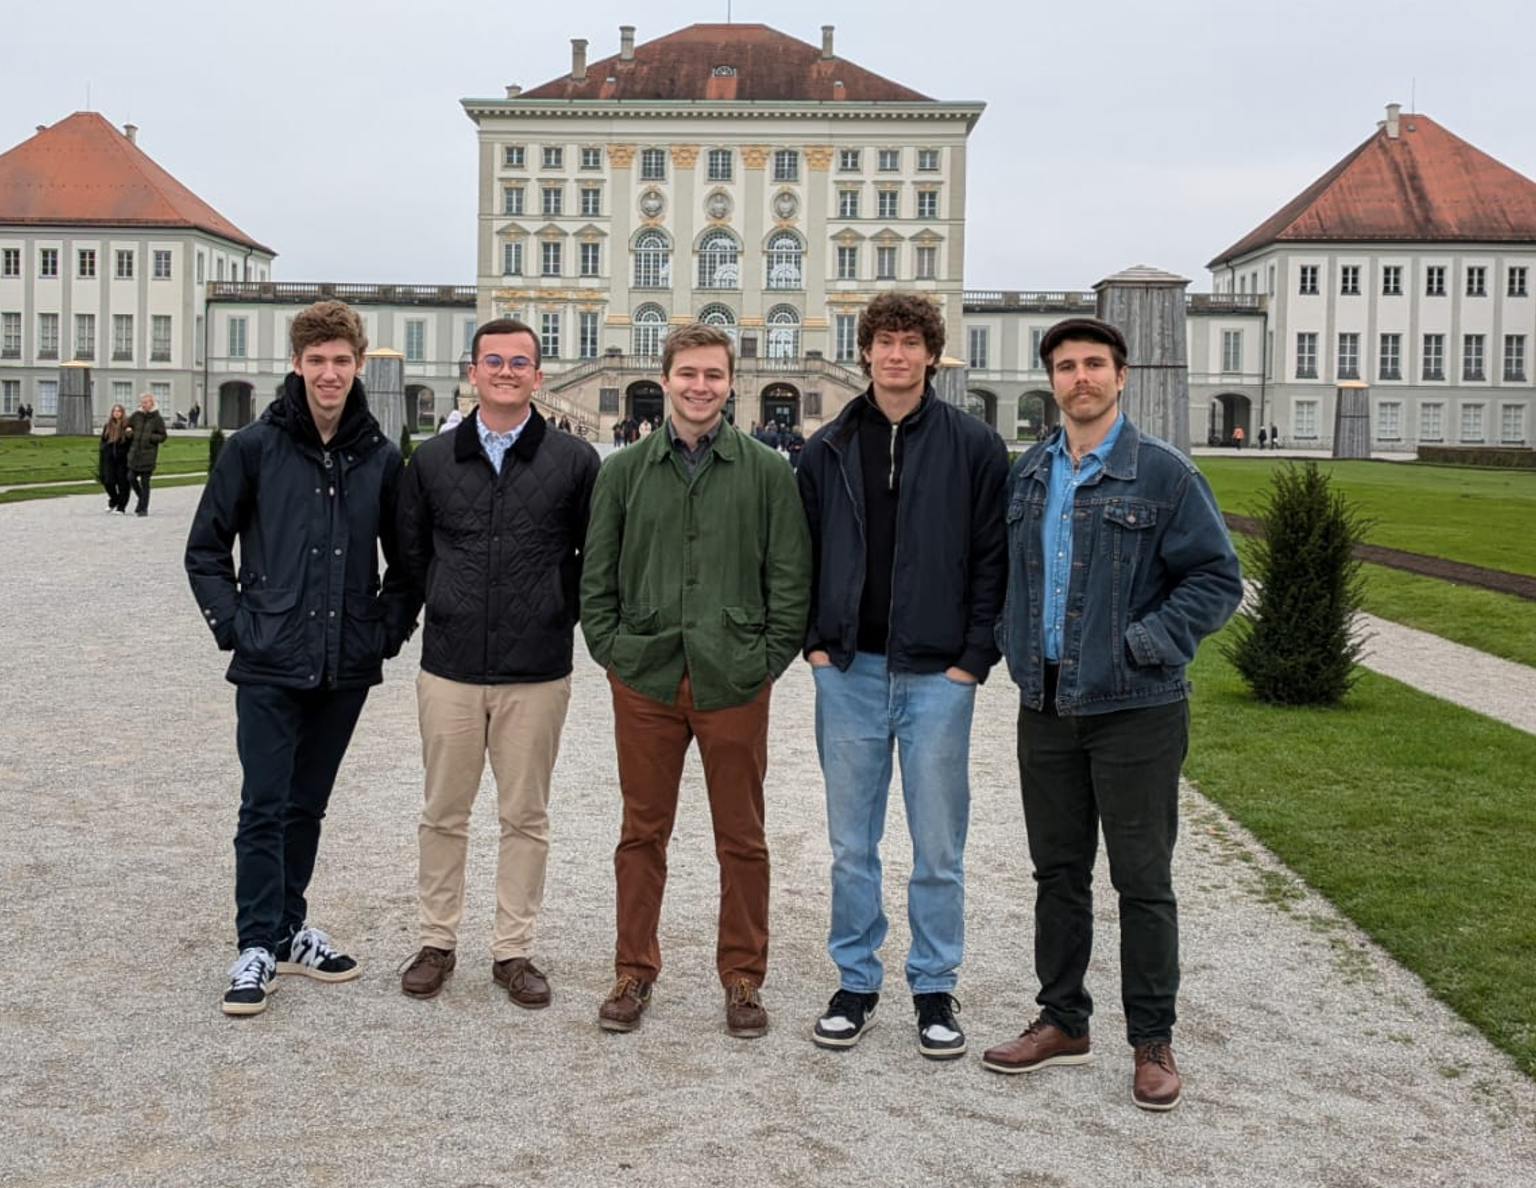
\includegraphics[width=.7\linewidth]{./Bilder/Neue Bilder/Aktivenfahrt/Aktivenfahrt}
		\end{figurehere}
\end{center}
	

\newpage

\section{Tanzen bei der KDStV Vandalia Prag zu
München im CV: Knotentanzkurs als perfekte Vorbereitung auf das Wintersemester}
\sectionmark{Knotentanzkurs}

	
\begin{multicols}{2}

Das Wintersemester der KDStV Vandalia war in diesem Jahr nicht nur akademisch,
sondern auch gesellschaftlich ein Highlight. Zahlreiche festliche Bälle und
Tanzveranstaltungen boten uns die Gelegenheit, das studentische
Verbindungsleben in voller Pracht zu genießen. Um bestens vorbereitet zu sein,
wurde an mehreren Abenden ein spezieller Knotentanzkurs angeboten. Dabei durfte
natürlich auch das ein oder andere Glas Sekt zur Einstimmung nicht fehlen!
\\
\\
\textbf{Der Knotentanz – Tradition mit Schwung}

Der Knotentanz ist eine besonders gesellige und kunstvolle Tanzform, die in
vielen studentischen Kreisen geschätzt wird. Er zeichnet sich durch kreative
Figuren und raffinierte Verknotungen der Tanzpartner aus, die sich am Ende auf
elegante Weise wieder lösen. Das Ergebnis ist eine dynamische Mischung aus
Geschick, Teamarbeit und viel Spaß.
\\
\\
\textbf{Die wichtigsten Figuren des Knotentanzes}

Während des Kurses lernten die Teilnehmer einige grundlegende Techniken, die
für den Knotentanz essenziell sind:

• Der Grundschritt: Eine fließende Bewegung im 3/4-Takt, die als Basis dient.

• Handwechsel: Durch das Wechseln der Hände entstehen die charakteristischen
Knotenfiguren.

• Drehungen: Mit einfachen oder mehrfachen Drehungen wird der Tanz fließender
und abwechslungsreicher.

• Die Schleife: Hier kreuzen sich die Arme der Tanzenden, was für optisch
beeindruckende Knoten sorgt.

• Verknoten und Entknoten: Der namensgebende Teil des Tanzes – durch geschickte
Bewegungen wird scheinbar ein chaotisches Muster erzeugt, das sich jedoch mit
der richtigen Technik elegant wieder auflöst.
\\
\\
\textbf{Ein Kurs mit viel Charme und Stil}

Über mehrere Abende hinweg konnten sich die Teilnehmer schrittweise verbessern
und ihr tänzerisches Können ausbauen. Besonders schön war die entspannte und
gesellige Atmosphäre, in der auch Anfänger schnell Fortschritte machten.\\
Die Kombination aus konzentriertem Üben und ausgelassener Stimmung machte den
Kurs zu einem Highlight des Semesters.\\
Dank des Knotentanzkurses konnten wir uns bestens auf die anstehenden Bälle
vorbereiten. Ob auf traditionellen Tanzveranstaltungen oder ungezwungenen
Feiern – unser erlerntes Können hat uns immer eine gute Figur machen lassen.

Wir freuen uns darauf, dieses Erlebnis im kommenden Semester zu wiederholen und
vielleicht noch weitere Tanzstile kennenzulernen.

	%
	\begin{flushright}
		\hfill\emph{Benedikt Kirchhof Va! xxx}
	\end{flushright}
	%	
\end{multicols}



\newpage

\section{Begrüßungsabend}
\sectionmark{Begrüßungsabend}

\begin{multicols}{2}
Am Freitag, dem 22. November, fand der Begrüßungsabend zum 120.
Gründungsfest am darauffolgenden Samstag statt, bei dem sich Damen, Freunde und
Gäste, geschätzte Alte Herren und deren Familien sowie Farben-, Cartell- und Bundesbrüder
in einer geselligen Runde zusammenfanden. Die Veranstaltung begann um 19 Uhr ct
im Festsaal der Verbindungsräumlichkeiten der K.D.St.V. Vandalia Prag zu
München im CV in der Friedrichstraße 34.

Nach der herzlichen Begrüßung aller durch den Organisator des Abends, den
damaligen Hohen Consenior Elia Strasser, und der Platzwahl begann der Abend mit
einer Vorspeise. Diesmal wurden die Teilnehmer des Abendessens von der Küche
mit Bruschetta und einem gemischten Salat verwöhnt. Während des Essens wurden
angeregte Gespräche geführt und Erinnerungen ausgetauscht. Nach einer schnellen
Erinnerung von Frau Chenu, auch ja die Immatrikulationsbescheinigungen
einzureichen, ging es mit guter Stimmung zum nächsten Gang.\\
Die Hauptspeise umfasste Reis mit Hühnerbrust auf Zitronen-Sahne-Sauce,
allerdings war der Reis zerkocht aufgrund von Problemen in der Küche. Berichten
zufolge hatte man dort mit der Sicherung zu kämpfen. Trotz dessen ließ sich
niemand die Laune verderben. Nach dem Hauptgang wurde ein Absacker in Form
eines Verdauungsschnapses von der Fuxia angeboten, welcher sehr gut ankam.\\
Die Atmosphäre war entspannt und herzlich, und man fühlte sich wohl. Die
Gespräche reichten von aktuellen Ereignissen bis hin zu der freudigen Erwartung
auf den morgigen Tag. Als runden Abschluss des Abends wurde als Nachtisch
Mousse au Chocolat mit roten Früchten serviert. Alle Gäste waren von der
gesamten Qualität der Speisen positiv überrascht, und es gab viel Lob für die
Köche.\\
Das ganze Drei-Gänge-Menü wurde von der Fuxia zu Tisch gebracht, und diese
versorgte auch alle mit Getränken, sodass es auch dahingehend nicht mangelte.
Außerdem bot sie Wein zum Verkauf an. Gegen 0 Uhr neigte sich der Abend dem
Ende zu, und alle gingen gesättigt und mit einem guten Gefühl im Bauch zu
Bette.

Insgesamt kann man nur noch allen Beteiligten und Mitwirkenden einen
herzlichen Dank für diesen wunderschönen, gemütlichen Abend aussprechen.

	%
	\begin{flushright}
		\hfill\emph{Jannis Jaschik Va!}
	\end{flushright}
	%	
\end{multicols}

\newpage

\section{Barrieren des Rauchstopps – Wenn der Glimmstängel mehr als nur Gewohnheit ist}
\sectionmark{Barrieren des Rauchstopps}

\begin{multicols}{2}
Manchmal sitzt man in Vorträgen und zählt
innerlich die Minuten bis zum Ende. Und manchmal – so wie bei Dr. Carsten
Schwindts Vortrag „Barrieren des Rauchstopps – Welche Rollen spielen
Alternativen“ – ist man plötzlich mitten in einer lebhaften Diskussion darüber,
warum man den Glimmstängel einfach nicht loslassen kann… und ob man es
überhaupt will.

Besonders spannend: Dr. Schwindt kam nicht
etwa als klassischer Anti-Raucher-Missionar daher. Nein, er vertritt Philip
Morris – genau die Firma, die an jeder verkauften Zigarette verdient. Ein
bisschen wie wenn der Fuchs einem den Hühnerstall erklärt. Aber Überraschung:
Er sprach erstaunlich offen und ehrlich über die Schattenseiten des Rauchens
und vor allem über die Stolpersteine beim Versuch, aufzuhören.

Ein Aha-Moment für viele im Raum: Das
Nikotin selbst ist nicht der Bösewicht. Zumindest nicht der
Hauptverantwortliche. Die wahren Übeltäter sind die zahllosen giftigen Stoffe,
die beim Verbrennen des Tabaks entstehen. Kurz gesagt – es ist nicht der Nikotinkick,
der schädigt, sondern der Rauch, der den Weg dorthin pflastert.

Und genau da setzt die Diskussion um
Alternativen an. Ob E-Zigaretten, Tabakerhitzer oder – der Publikumsliebling im
Vortrag – Snus. Bei letzterem wurden einige Ohren besonders groß. „Moment, das
ist doch illegal in Deutschland, oder?“ – fragte jemand. Dr. Schwindt klärte
lässig auf: Kaufen? Nein. Konsumieren? Ja. Willkommen im rechtlichen
Graubereich!

Aber der wahre Star des Tages war
eigentlich das Publikum selbst. Die Diskussion mit den Rauchern im Raum hatte
fast schon therapeutischen Charakter – irgendwo zwischen ehrlicher
Selbsterkenntnis und leichtem Trotz. Da wurden Strategien geteilt, Ausreden
gefunden („Rauchen entspannt halt einfach!“) und ganz nebenbei auch ein paar
Mythen entzaubert. Man spürte förmlich, wer innerlich gerade einen Pakt mit
sich selbst schloss: „Okay, vielleicht versuche ich’s nochmal mit dem Aufhören…
irgendwann… vielleicht morgen.“

Dr. Schwindt hat es geschafft, die
Thematik mit einer Mischung aus Fachwissen, Offenheit und einer Prise Humor zu
beleuchten. Ohne erhobenen Zeigefinger, aber auch ohne zu verharmlosen. Ein
Vortrag, der nachwirkt – und bei dem am Ende vermutlich einige den Raum
verließen mit dem Gedanken: „Vielleicht ist es doch Zeit, sich von der Kippe zu
trennen. Oder zumindest mal eine Pause zu machen.“

Und wenn nicht? Dann wissen wir jetzt
zumindest, dass es mehr Alternativen gibt als nur Kaugummis und Pflaster. Und
vielleicht reicht ja genau dieser Gedanke, um irgendwann den entscheidenden
Schritt zu wagen.

Lieber Dr. Carsten Schwindt, vielen lieben
Dank für den interessanten Vortrag! Man sagt, der ein oder andere Bundesbruder
hat sich vom Rauchen getrennt – zumindest im nüchternen Zustand! Und das ist
doch schon mal ein guter Anfang!

	\begin{flushright}
		\hfill\emph{Elias Haindl Va!}
	\end{flushright}


\end{multicols}


\newpage

\section{Wertschöpfung und Kreativität: Einblicke in das geistige Eigentum}
\sectionmark{Einblicke in das geistige Eigentum}

\begin{multicols}{2}
Geistiges Eigentum ist ein Thema, das oft
abstrakt wirkt – doch der Vortrag von Leo, einem auf dieses Gebiet
spezialisierten Juristen, bewies das Gegenteil. Unter dem Titel „Wertschöpfung
und Kreativität: Geistiges Eigentum und seine Bedeutung“ führte er sein
Publikum durch die komplexe, aber hochrelevante Welt der Urheberrechte,
Lizenzen und Schutzmechanismen für kreative Werke.

Besonders bemerkenswert war die Art der
Präsentation: Statt eines trockenen Monologs gestaltete Leo seinen Vortrag
interaktiv und ließ Raum für Fragen aus dem Publikum. Diese Möglichkeit, direkt
ins Gespräch zu treten, machte die Veranstaltung nicht nur lebendig, sondern
auch besonders lehrreich. Sein humorvoller Stil sorgte zudem für eine lockere
Atmosphäre – ein angenehmer Kontrast zu einem Thema, das oft mit Paragraphen
und juristischem Fachjargon assoziiert wird.

Als Kunststudent habe ich mit besonderem
Interesse zugehört, denn die Frage nach dem Schutz kreativer Arbeit betrifft
mich als Künstler unmittelbar. Welche Rechte habe ich an meinen Werken? Wie
kann ich sie wirtschaftlich nutzen, ohne ihre künstlerische Integrität zu
gefährden? Solche Fragen wurden praxisnah und verständlich beleuchtet.

Lieber Leo, abschließend bleibt mir nur,
mich für diesen bereichernden und inspirierenden Vortrag zu bedanken. Die
Mischung aus Fachwissen, Humor und Dialog hat gezeigt, dass geistiges Eigentum
alles andere als trocken ist und dass es sich gerade für Kunstschaffende lohnt,
sich intensiv damit auseinanderzusetzen (auch wenn die Anzahl der Vandalen
nicht allzu groß ist…).

Vielleicht bis bald auf einer Ausstellung für
zeitgenössische Kunst! :D
\end{multicols}

\begin{flushright}
		\hfill\emph{Elias Haindl Va!}
	\end{flushright}
	%	
			

\newpage


\input{Artikel/artikel_Brauereiführung}
\newpage

\input{Artikel/Bilder_Brauereiführung}
\newpage

\section{Trauerkneipe}

\sectionmark{Trauerkneipe}


Liebe Bundesbrüder,
\begin{multicols}{2}
Heute haben wir uns hier versammelt, um allen Bundesbrüdern zu gedenken,
die im letzten Jahr von uns gegangen sind.\\
Der recht bekannte Auszug aus der Bibel zeigt uns als katholische
Verbindungsstudenten, dass wir, egal wie finster die Zeit auch scheinen möge,
unserem Herrn vertrauen können, dass er ein nie erlöschendes Licht in unserem
Herzen ist. Dieser Halt hilft uns, durch schwere Zeiten zu gehen, denn wir
wissen, wir sind nie allein. Als Vandalia stehen wir nicht nur in Gemeinschaft
mit Gott, sondern sind auch in Gemeinschaft mit allen Vandalen im Lebensbund
verbunden. Dieser Lebensbund verbindet jeden von uns, vom frisch rezipierten
Fux bis zum hoch betagten Alten Herrn. Generationenübergreifend stehen wir für
gemeinsame Werte und Prinzipien. Diese prägen uns und machen uns zu dem, was
wir sind. Auch wenn wir mit jedem neuen Fuxen den Lebensbund in freudiger
Stimmung erweitern, so macht es doch auch jedes Mal aufs Neue betroffen, wenn
ein Bundesbruder aus diesem Lebensbund von uns geht.

Im vergangenen Jahr mussten wir die Bundesbrüder

Dipl. Kfm. (Diplom-Kaufmann) Karl Jähn v/o Kalle,

StD a.D. (Studiendirektor) Roland Kurz v/o Stunk und

Dr. med. (Doktor med.) Kurt Bröckner v/o Stachus

in die Hand Gottes geben.

Auch wenn wir als junge Vandalen oft keinen direkten Bezug zu den
Verstorbenen haben, so saß doch jeder von ihnen schon einmal an einem eurer
Plätze, ging auf Convente, Kneipen und Kommerse, brachte sich in der Verbindung
ein, war einer von uns.\\
Dieses Gleichbleiben der gemeinsamen Traditionen wird einem im Gespräch mit
jungen und älteren Philistern immer wieder klar.\\
Bei einigen von uns gegangenen Bundesbrüdern zeigen wir ein letztes Mal
unseren Respekt und so auch die Verbundenheit zur Vandalia. Manchmal geht diese
Verbundenheit über die Bundesbrüderlichkeit hinaus. So auch vor gut einem
halben Jahr, als wir an der Beerdigung von Ute Fest teilnahmen, die am 23. Juli
2024 verstorben ist. Auch sie stand unserer Verbindung nahe, genauso wie die
Bundesbrüder, die von uns gingen.

So nehmen wir heute Abschied von unseren verstorbenen Bundesbrüdern, die
für viele Vandalen gute Freunde auf ihrem Lebensweg waren.

\end{multicols}

	\begin{flushright}
		\hfill\emph{Raphael Frank Va! x}
	\end{flushright}
	%	

\newpage

\section{Der singfähige Vandale}
\sectionmark{Der singfähige Vandale}

%\begin{figurehere}
%	\begin{center}
%		\includegraphics[width=\linewidth]{Bilder/andechs2.jpg}
%%		\caption{xxx} 
%	\end{center}
%\end{figurehere}

\begin{multicols}{2}
	
	Die Singfähigkeit des Vandalen zu garantieren ist seit jeher Aufgabe des Fuxmajors. In seinen Fuxenstunden klärt er nicht nur über die historischen Hintergründe der Verbindung auf, er bringt dem Fux auch das Vandalische Liedgut nahe. 
	Desweiteren steht es aber in der Verantwortung jedes Bundesbruders, auf den Kommersen das Liedgut weiterzugeben. Denn bei vielen der Kommers- und Kneipen-Schlager finden sich Eigenheiten, die nicht so im Notentext notiert sind. Ein Beispiel ist das furios-schnelle Ende bei “Ich schieß’ den Hirsch”. Auch die Zwischenrufe im “Münchner Lied” sind solche Eigenheiten, die man erst nach mehrmaligem Hören lernt und vielleicht sogar verändert (Da die Biergeschmäcker doch recht unterschiedlich sind.)
	
	Doch Singen ist mehr als nur das CV-Liederbuch auswendig zu kennen. In meinem Gesangsunterricht an der Musikhochschule arbeiten wir ständig an Intonation, Vokalfarbe, Interpretation, Phrasierung und Atmung, dem Fundament des Singens.
	Dies sprengt den Umfang des Machbaren für einen Hobby-Kneipensänger – oder tut es das? Einen Vorteil hat die feierliche Stimmung des studentischen Beisammenseins: die körperliche Aktivierung. Wie schon erwähnt, ist die Atmung das Fundament. Dazu gehört das Einatmen tief in den Bauch (Zwerchfell) und die Ausatemmuskulatur (seitliche Bauchmuskulatur), die den Klang verstärkt. Beim Lachen werden dieselben Regionen aktiviert, und jede gute Kneipe sollte hierzu genug Möglichkeiten schaffen.
	
	Der Vollständigkeit halber hier aber doch ein Tipp für den fleißigen Sänger. Nehmen wir nochmal den “Hirsch”. Wenn du das Wort “schieß” sprichst, was passiert mit deinen Mundwinkeln? Gehen sie intuitiv zur Seite, wie wenn du grinsen würdest?
	Beim Singen ist vor allem das Formen der Vokale wichtig, da diese den Klang beinhalten. Nimm also die Mundform des “sch”, die sogenannte Schnute (oder wie man es 2014 auf Instagram nannte: Duckface. Spreche nochmal \glqq schieß\grqq, ohne dabei die Schnute zu verändern. Merkst du den dunkleren Klang? Spreche es nochmal, spanne dabei deinen Bauch an und stell dir vor, wie ein dicker Opernsänger sprechen würde.
	
	Zum Abschluss darf ich darauf verweisen, dass das Singen auf keinen Fall zu akademisch werden soll. Vor allem in die Kneipe passt das, wie ich finde, nicht. Die Energie einer Kneipcorona habe ich in meiner Chorerfahrung bisher nur ganz selten genauso gespürt, auch beim Singen in den großen Konzerthäusern in Hamburg und Berlin zum Beispiel nicht immer.
	Deshalb darf ich getrost sagen, dass ich mir über die sängerische Zukunft unserer Vandalia keine Sorgen mache. 
	
	Wer sich gerne darüber hinaus an neuen Herausforderungen probieren möchte: Ich lade euch herzlich zum Chor der Prager Universitäts-Sängerschaft Barden ein, den ich seit zwei Jahren leite. Die Probe findet immer montags um 19.00 Uhr in der Leopoldstraße 255 statt.
	
	%
	\begin{flushright}
		\hfill\emph{Vincent Penschke Va! }
	\end{flushright}
	%	
\end{multicols}
%
%\begin{figurehere}
%	\begin{center}
%		\includegraphics[width=.8\linewidth]{Bilder/pios2}
%		\caption{Realer Aufbau} 
%	\end{center}
%\end{figurehere}
\newpage

\section{Neubewertung des Fuxendaseins}
\sectionmark{Neubewertung des Fuxendaseins}

%\begin{figurehere}
%	\begin{center}
%		\includegraphics[width=\linewidth]{Bilder/andechs2.jpg}
%%		\caption{xxx} 
%	\end{center}
%\end{figurehere}

Was ist der Fux?

Dummfux. Kackfux. Fux: Stoff!

\begin{multicols}{2}
Es gibt nicht viel zu beneiden in manchen Momenten an der Art und Weise wie man als Fux behandelt wird. Man ist nicht da, mit den anderen auf gleicher Augenhöhe, sondern ist eine Stufe darunter, führt die niedrigen Arbeiten aus, wartet auf die Erlösung seiner Schicht.
Das Fuxendasein darf sich emanzipieren. Es sind nicht wir Burschen, die der Verbindung seinen Gehalt geben, sondern eine Verbindung wächst und gedeiht, verblüht und erkrankt am neuen Zustrom seiner Mitglieder. Der Fux ist kein Mitglied auf Probe. Er stellt die Verbindung auf die Probe. Es liegt an ihm, ob er entscheidet uns aufzuwerten oder durch seine Abkehr wieder in die Mittelmäßigkeit zu verstoßen. Für uns bleibt es nur zu warten, wie er sich entscheidet, es darf uns genügen den Rahmen zu bilden für die Entscheidung eines Menschen, der noch keine Abhängigkeit von uns erfährt.
Der Fux ist das zukünftig Kommende. Was die Verbindung in einigen Jahren ist, das liegt alles im Fux jetzt verborgen und wachsend. Es liegt an uns dem Fux zu dienen in der Weise, dass wir nicht großspurig ihm die Welt und das Verbindungsdasein erklären und verkünden. Es liegt an uns die Welt und das Verbindungsdasein in einer Weise zu strukturieren und zu verändern, die dem Fuxen seinen freien Lauf gewährt. Er bedarf der Freiheit sich umzublicken, unbedrängt die Räume zu erkunden und in seiner Rolle als der Neue von Repressalien frei zu bleiben.
Der Fux bedarf unseres höchsten Respekts. Nicht weil er neu ist, sondern weil er das ist, was die Verbindung sein wird. In ihm spiegelt sich auch das, was wir im Moment leisten. Die Qualität des Verbindungswesens hat sich schon immer an der Höflichkeit, Zwischenmenschlichkeit und dem Respekt gezeigt, mit dem wir einander auf Augenhöhe begegnen. Wer davon nichts weiß, dem ist die Idee der Brüderlichkeit zugunsten einer ungleichen Hierarchie verlorengegangen. In einem solchen Raum, der den Fux als Bundesbruder zweiter Klasse betrachtet, hat die Zukunft auch nichts verloren. Es gibt hier nichts zu holen für den Fuxen. Weshalb sich einer Gemeinschaft anschließen, die keinen Respekt für niedere Tätigkeiten hat? Weshalb der Unverschämtheit und Arroganz, die einem entgegengebracht wird, mit Offenheit und Zuversicht, dass es sich ändern würde, entgegentreten? Es gibt für den Fuxen nur etwas zu holen, wenn wir ein Raum sind und werden, in dem Hierarchie als etwas gezeichnet wird, das als Tätigkeitsverteilung, aber nicht als Klassenunterschied das Verbindungsleben strukturiert. Nicht jeder erfüllt dieselbe Aufgabe, aber jeder ist als Gleicher an der Verbindung beteiligt. Dass der Fux noch vor dem langfristigen Beitritt zur Verbindung steht, ist Aufgabe für uns, ihm zu zeigen, was es heißt, bereits jetzt einer von uns zu sein.
Ein Bruder zu sein, ist nicht einfach. Jeder mit Geschwistern weiß das. Sich das Wort Brüderlichkeit so zur Aufgabe zu machen, wie Verbindungen es tun, muss für uns heißen:
\begin{itemize}
    \item Leben auf selber Augenhöhe, ohne bösen Willen einander.
    \item Eingeständnis, dass wir dieselben Gerechtigkeitsansprüche haben, dasselbe Recht auf Wohlwollen und Respekt.
    \item Ermöglichung eines sinnvollen und erfüllenden Beitrags zum gemeinschaftlichen Leben. Hierarchie wo es nötig ist, aber nicht, wo es schadhaft ist.
\end{itemize}
Das, was ich heute als Verbindungsstudent bin, bin ich zum großen Teil geworden während der Fuxenzeit. Was mich an der Verbindung hält, stammt aus dieser Zeit. Was ich dem Neuen schulde, ist dieselbe Freiheit und Gleichheit, die mir an vielen Stellen entgegengekommen ist, und die mich bewogen hat, das Schlechte in Kauf zu nehmen. Wer die Verbindung ändern will, der bedarf des Fuxen.
	\begin{flushright}
		\hfill\emph{Christian Schnurr Va! }
	\end{flushright}
	%	
\end{multicols}
%
%\begin{figurehere}
%	\begin{center}
%		\includegraphics[width=.8\linewidth]{Bilder/pios2}
%		\caption{Realer Aufbau} 
%	\end{center}
%\end{figurehere}
\newpage

%%%%%%%%%%%%%%%%%%%%%%%%%%%%%%%%%%%%%%%%%
%% Vortraege

%\clearpage

%%%%%%%%%%%%%%%%%%%%%%%%%%%%%%%%%%%%%%%%%%%%%%%%%
%% Nachrufe
%\section{Trauerkneipe}


\begin{multicols}{2}
	%
	
	\begin{flushright}
		\hfill\emph{Va! x}
	\end{flushright}
	%
\end{multicols}



%\clearpage

%\clearpage

%%%%%%%%%%%%%%%%%%%%%%%%%%%%%%%%%%%%%%%%%%%%%%%%%
%% Todesanzeigen

\newpage
%\section*{Todesanzeigen}
\sectionmark{Todesanzeigen}

% Set thickness and padding of the frame
\setlength{\fboxsep}{3pt}  % No padding between the image and the frame
\setlength{\fboxrule}{1mm} % Thickness of the frame

%\begin{figure}[h!]
%	\begin{center}
%		\fbox{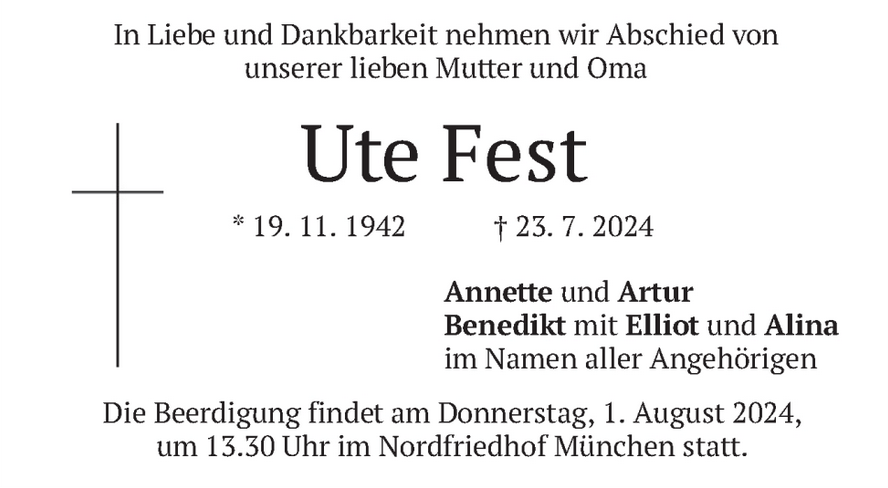
\includegraphics[width=.7\linewidth]{./Todesanzeigen/23.07.2024 Ute Fest.png}}
%		\vspace*{0.5cm}
%		\fbox{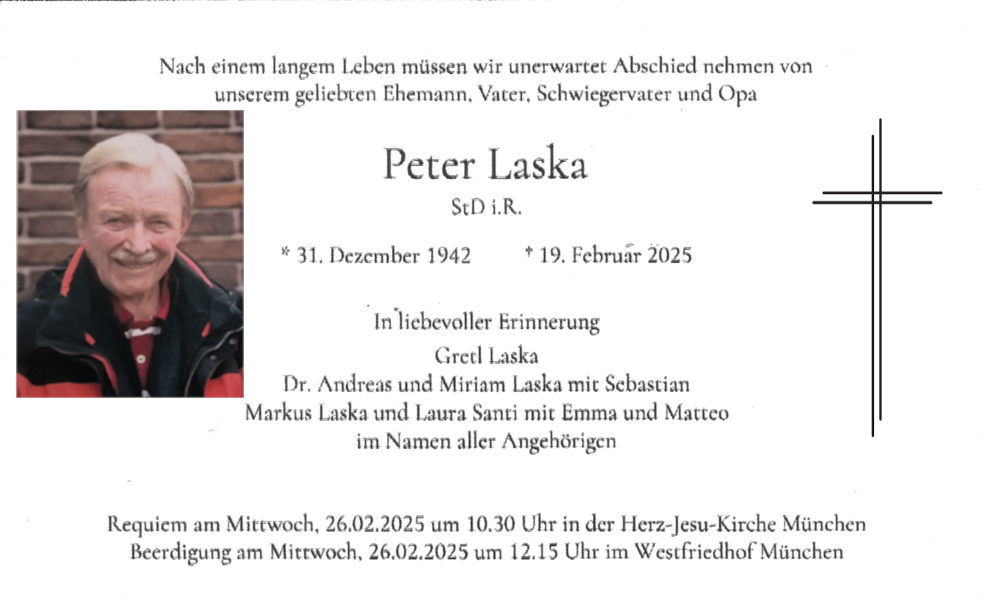
\includegraphics[width=.7\linewidth]{./Todesanzeigen/19.02.2025 PeterLaska.png}}
%	\end{center}
%\end{figure}
\begin{figure}[h!]
    \centering
    \fbox{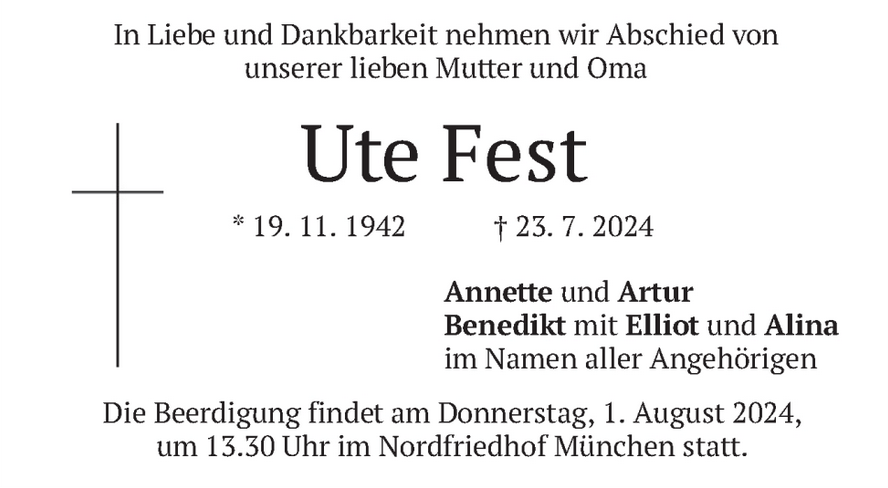
\includegraphics[width=.7\linewidth]{./Todesanzeigen/23.07.2024 Ute Fest.png}}
\end{figure}
    \vspace{0.4cm} % Should work better
\begin{figure}[h!]
    \centering
    \fbox{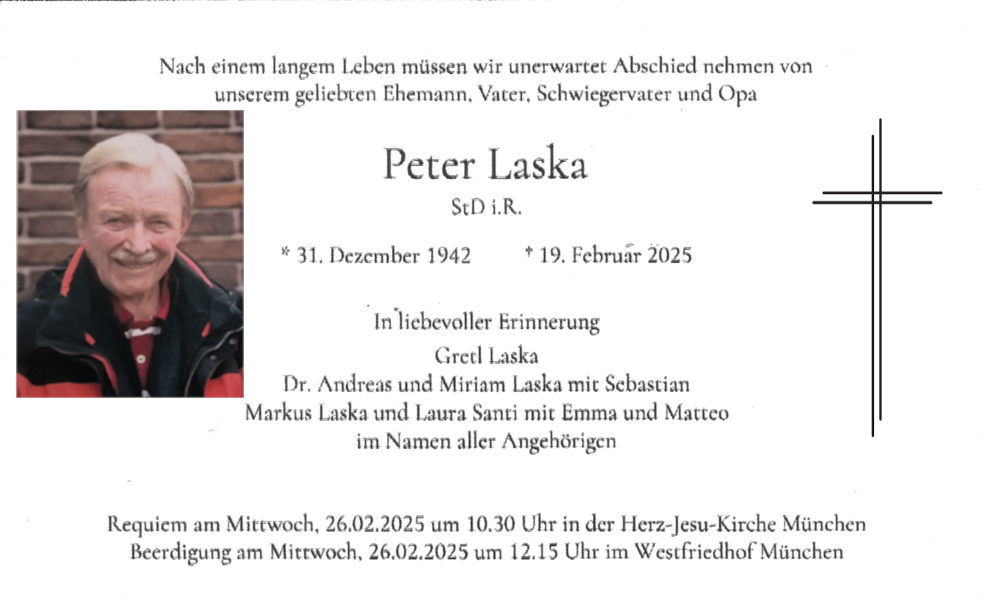
\includegraphics[width=.7\linewidth]{./Todesanzeigen/19.02.2025 PeterLaska.png}}
\end{figure}

\begin{multicols}{2}
			Am 26 Februar 2025 wurde unser Bundesbruder Peter Laska, StD i.R., im Familiengrab im Münchner Westfriedhof beigesetzt.
			Hier ruht auch sein Vater, unser hochverdienter Bundesbruder Josef Laska.
			Drei Chargierte der Aktivitas und einige Bundesbrüder erwiesen ihm die letzte Ehre und gaben ihm Band und Mütze als
			Dank und Zeichen der Verbundenheit mit ins Grab.
			Bundesbruder Peter Laska, geb. 1942 in Böhmen, wurde am 13.11.1964 von Vandalia rezipiert.
			Im WS 1965 war er Consenior der Aktivitas, 1966 Senior.
			Im Mai 1975 philistriert, übernahm er dennoch das anspruchsvolle Amt des Jubelseniors - 70 Jahre Vandalia! -
			 im Sommersemester 1975, um danach das Amt des Philisterconseniors weiterzuführen.
			61 Jahre lang hat Bbr. Peter Laska Vandalia die Treue gehalten. Ihm gebührt Vandalias besonderer Dank.
			REQUIESCAT IN PACE!
			\begin{flushright}
			\hfill\emph{Bernhard Müller Va!}
			\end{flushright}
\end{multicols}

\clearpage



%%%%%%%%%%%%%%%%%%%%%%%%%%%%%%%%%%%%%%%%%%%%%%%%%
%% Vandalia gratuliert
\section*{Vandalia gratuliert}
\sectionmark{Vandalia gratuliert}

{\footnotesize

\begin{multicols}{2}
	
%\textbf{zum 20. Geburtstag}\\


%\textbf{zum 30. Geburtstag}\\


\textbf{zum 40. Geburtstag}\\
Gabriel Lederle (12.04.1985)
\\



%\textbf{zum 50. Geburtstag}\\    Für spätere verwendung da niemand WS2024-2025 50 geworden ist




\textbf{zum 60. Geburtstag} \\
Alexander Huber (24.05.1965)\\
Stefan Guggenmos (13.05.1965)\\


% \textbf{zum 70. Geburtstag}\\ Siehe oben


%\textbf{zum 75. Geburtstag}\\ Siehe oben




\textbf{zum 80. Geburtstag}\\
Elmer Weisshuhn (10.04.1945)\\
Johann Berger (01.03.1945)\\
Wolfgang Bouché (28.02.1945)\\
Wolfgang Schorn (21.02.1945)\\

%\textbf{zum 85. Geburtstag}\\



\textbf{zum 90. Geburtstag}\\
Konrad Mayer (24.05.1935)\\
Richard  Strobel (05.05.1935)\\

\columnbreak

\textbf{zum 95. Geburtstag}\\
Ferdinand Stocker (17.03.1930) \\


%\vspace{1.5mm}

%\textbf{zur Vaterschaft}\\


\textbf{zur Hochzeit}\\
Bundesbruder Anton Brandl und seiner Frau Corina
zur Hochzeit am 28.12.2024
%\textbf{zur Geburt}\\


\vspace{1.5mm}

%\textbf{zur Philistrierung}\\


%\textbf{zur Burschung}\\


%\textbf{zur Promotion}\\

%\textbf{zum 100 Semesterband}\\

\textbf{zur Philistrierung}\\
SoSe 2023:\\
Janosch Christ\\
Martin Kölbl\\
\newline
WiSe 2023/24:\\
Philip Levi


\vspace{1.5mm}



%\textbf{ZMer im Sommersemester}\\


%\vspace{5mm}
%\vbox{
%	\textbf{Chargenkabinett des SS 20}\\[0.5ex]
%	\begin{tabular}[h]{rl}
%		X     & Korbinian Heinrich \cr
%		FM    & Felix Fisel \cr
%		XX    & Noel Riedl \cr
%		XXX   & Elias Baumgartner \cr
%		XXXX  & Andreas Mayerhofer \cr
%	\end{tabular}
%}



\end{multicols}


\vspace{1cm}

\begin{multicols}{2}

%\vspace{6pt}
%\vfill
%\vspace{12pt}
%\vspace{5pt}

\vbox{
\textbf{Chargenkabinett des WS24/25}\\[0.5ex]
\begin{tabular}[h]{rl}
	X     & Raphael Frank \cr
	FM    & Magnus Weig \cr
	XX    & Elia Strasser \cr
	XXX   & Benedikt Kirchhof \cr
	XXXX  & Felix Hantke \cr
\end{tabular}
}

\end{multicols}                                                                                       

%\vfill

%\begin{figurehere}
%  \begin{center}
%    \includegraphics[width=\hsize]{Bilder/ChC_SS11.jpg}
%    \caption{Das Chargenkabinett Vandaliae im Sommersemester 2011}
%  \end{center}
%\end{figurehere} 
}



\end{document}
